%%%%%%%%%%%%%%%%%%%%%%%%%%%%%%%%%%%%%%%%%%%%%%%
\chapter{Communication Chain} 
\label{chap:commchain}
%%%%%%%%%%%%%%%%%%%%%%%%%%%%%%%%%%%%%%%%%%%%%%%
\graphicspath{{C:/Users/Kevin/Bachelarbeit/Bachelorarbeit/01_Bachelorarbeit_LaTex/02_Figures/}}


First, the communication chain for simulations is introduced in Figure 2.1. The link is built up of three main blocks: Transmitter, channel, and receiver. The transmitter contains the encoder, interleaver, and mapper. We start with feeding a random generated bit stream, representing a message, \underline{U} into the encoder. The resulting encoded code word \underline{C} is next processed in the interleaver producing the shuffled code word \underline{C}'. The mapper can now modulate \underline{C}' into the desired modulation scheme with the symbol frame \underline{X}. In the channel various kind of noises and fading can be added to the modulated signal,\,e.g., \gls{AWGN}. Next the receiver, consisting of the counterparts build in the transmitter, will first demap the signal \underline{Y} to the estimated code word \underline{$\hat{\textrm{U}}$}. After de-interleaving and decoding the transmitted symbol an estimate \underline{$\hat{\textrm{U}}$} is determined. In the simulation we will compare the estimated \underline{$\hat{\textrm{U}}$} with the initially created input message \underline{U} to calculate the error rate in the system.
\begin{figure}[!htb]
	\centering
	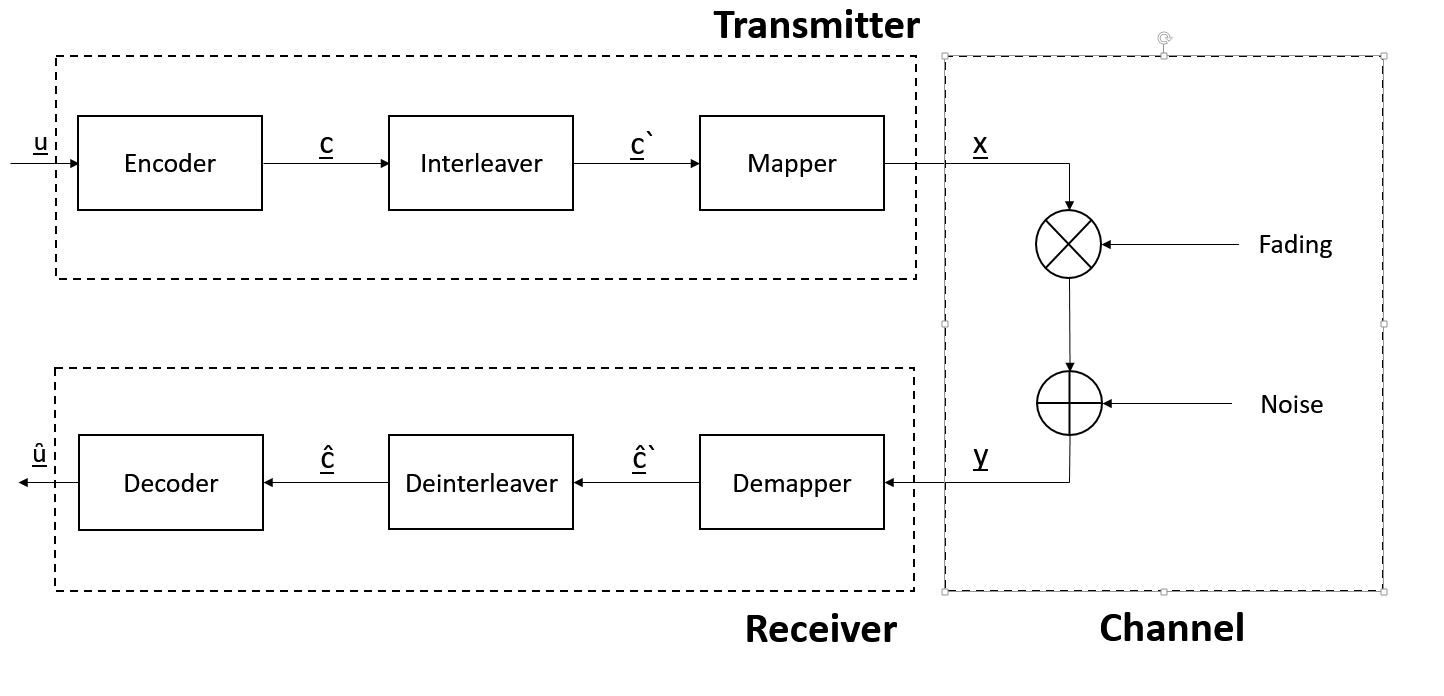
\includegraphics[width=0.95\textwidth]{Channelmodel.PNG}
	\caption{Communication chain for simulation}
	\label{fig:commchain}
\end{figure}

\section{Encoder/Decoder}
\label{sec:enc}

There are many ways to make the transmission more stable and less error prone. A major role in this protection plays the encoder and its counterpart the decoder. Encoder/decoder come in many different forms and shapes,\,e.g., as pre-built circuits in systems but more commonly today in form of coder performed as software with the help of CPUs. They reach from simple linear block codes to more complex convolutional codes to the latest turbo codes. It is also important to note, that one coder working well in \gls{AWGN} channel will often not have the same performance in a fading channel \cite[p.~262]{Goldsmith08}.
\newline
A further look will be taken into \gls{LDPC} codes, in particular the WiMax code. While \gls{LDPC} was mainly ignored in the past, since the 1999's the introduction of turbo codes and a sharp increase in computing power helped the recognition of these forms of channel coding.
\newline
\gls{LDPC} codes are linear block codes with a particular structure for their parity check matrix \textbf{H}. In the case of \gls{LDPC} codes \textbf{H} has only a small amount of nonzero entries, which means that there is a low density in the parity check matrix.
Another important difference in LDPC to turbo codes is the complexity of encoding and decoding. While turbo codes have low complexity in encoding they have high complexity in decoding. The total opposite can be said about \gls{LDPC} with high complexity in encoding and low complexity in decoding.  
\newline
WiMax, based on the IEEE 802.16 standard \cite{WiMaxTech}, is a broadband wireless technology used in small and medium distances in urban areas. It should be noted, that for WiMax codes there are predefined code lengths, code rates and encoding classes. Code lengths can range from 576 bits up to 2034 bits. Code rates are divided into four rates\footnote{$R = \frac{\textrm{number of data bits in a message}}{\textrm{number of bits in the codeword}} $}: 1/2, 2/3, 3/4, 5/6. Also the code is divided into two encoding classes A and B, which only A will be used in the simulations \cite{WIMAX}.
\newpage

\section{Bit interleaver/De-interleaver}
\label{sec:interleaver}

While the above mentioned \gls{LDPC} codes (Chapter \eref{sec:enc}) work really well on its own this is not always the case. Therefore another important block must be included in this channel. To guarantee a stable performance the method of interleaving will be introduced. Interleaving will handle a major problem in an AWGN and fading channels, namely the appearance of burst errors. In an \gls{AWGN} channel burst errors happen for modulation schemes, which assign long bit streams to a constellation symbol,\,e.g. 64-QAM. These long bit sequences can be made unrecognizable by high noise interference. In the fading channel burst errors are caused by deep fading over a set time in the transmission of the code word. \gls{LDPC} coding suffers from loss of performance trying to correct these burst errors, deteriorating even more with the increase of the burst error length. On the other hand \gls{LDPC} codes are very efficient in decoding codewords with uniformly distributed errors in the codeword. With the interleaver the code word will be shuffled into a new code word, uniformly distributing the burst errors. At the receiver a restoration of the shuffled code word back into its initial state will take place (\fig{fig:interleaver}).
\begin{figure}[!htb]
	\centering
	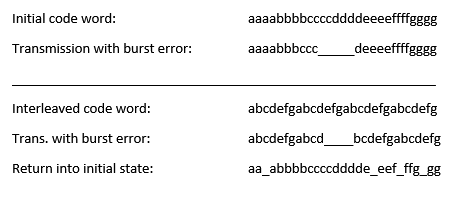
\includegraphics[width=0.8\textwidth]{interleaver.png}
	\caption{Example for interleaving}
	\label{fig:interleaver}
\end{figure}

As clearly seen in \fig{fig:interleaver} the interleaver will not remove any errors but will prevent or at least mitigate the presence of burst errors. The \gls{LDPC} decoder can correct single errors again. There are two main methods of interleaving today: symbol-interleaved coded modulation (SICM) will interleave the symbols after the modulator while \gls{BICM} will interleave the single bits before the modulator block. \gls{BICM} will be used in this thesis for having a more dominant position in practical communication systems \cite{Fabregas03}.

\clearpage

\section{Mapper/Demapper}
\label{sec:mapper}

In this block the mapper, also called the modulator, makes it possible to create a sequence of symbols out of the codeword. Group of bits are taken from the bit stream to combine them to specific constellation symbol. The symbols are located in a real/imaginary plane, also called Inphase/Quadrature planes (I/Q-planes). With the distance from the null point of the axis giving us the magnitude of the signal and the angle to the real axis the phase shift. 
\begin{figure}[!htb]
	\centering
	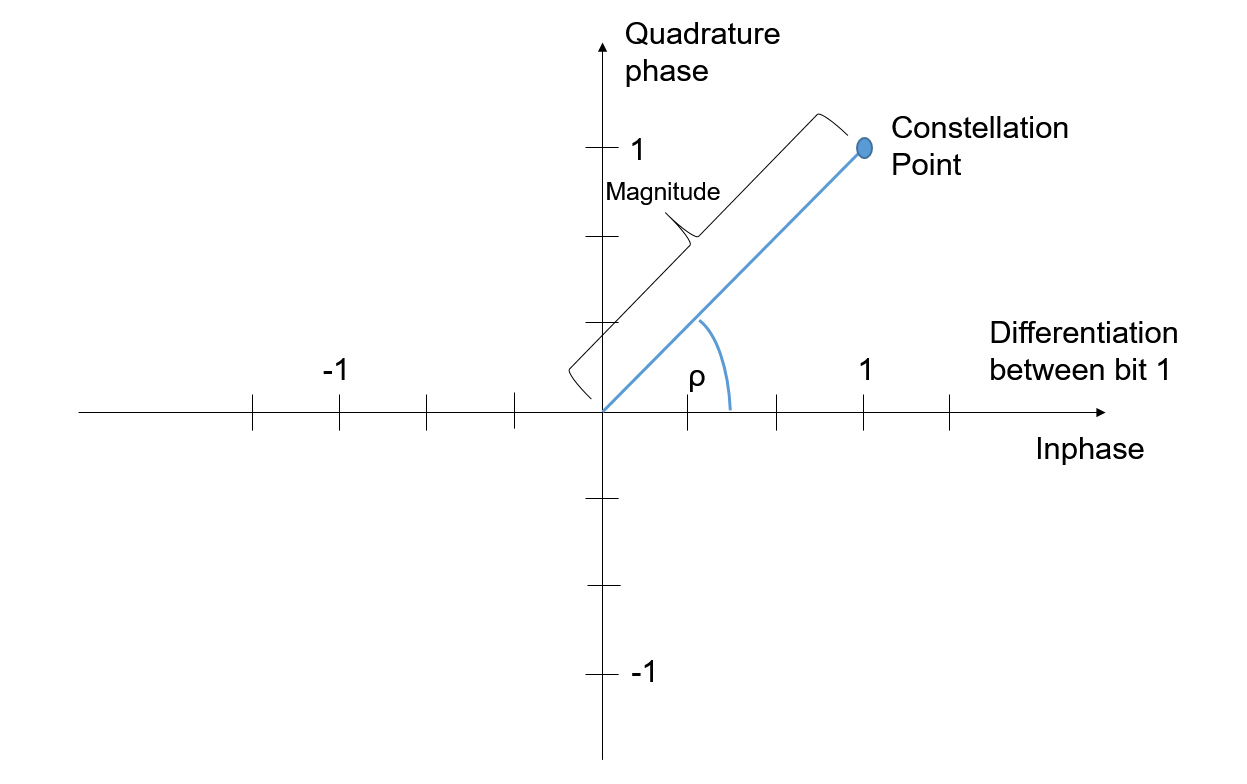
\includegraphics[width=0.8\textwidth]{IQ.png}
	\caption{Example for constellation point with amplitude and phase shift angle ($\phi$)}
	\label{fig:IQ}
\end{figure}

There are many forms of modulation schemes, with the most common ones being M-phase shift keying (PSK), M-frequency shift keying (FKS), M-amplitude modulation (AM) and M-\gls{QAM}. For the simulation, a further look will be taken at \gls{QPSK}, 16-\gls{QAM} and 64-\gls{QAM}, which are all depicted in \fig{fig:Modulation}.

\begin{figure}[!htb]
	\setlength\fwidth{0.4\textwidth}
	\setlength\fheight{0.3\textheight}
\begin{subfigure}
	
		% This file was created by matlab2tikz.
%
%The latest updates can be retrieved from
%  http://www.mathworks.com/matlabcentral/fileexchange/22022-matlab2tikz-matlab2tikz
%where you can also make suggestions and rate matlab2tikz.
%
\begin{tikzpicture}

\begin{axis}[%
width=\fwidth,
height=\fheight,
at={(0\fwidth,0\fheight)},
scale only axis,
xmin=-4,
xmax=4,
xtick={-8, -7, -6, -5, -4, -3, -2, -1,  0,  1,  2,  3,  4,  5,  6,  7,  8},
xlabel style={font=\color{white!15!black}},
xlabel={I},
ymin=-4,
ymax=4,
ytick={-8, -7, -6, -5, -4, -3, -2, -1,  0,  1,  2,  3,  4,  5,  6,  7,  8},
ylabel style={font=\color{white!15!black}},
ylabel={Q},
axis background/.style={fill=white},
title style={font=\bfseries},
title={QPSK Modulation},
xmajorgrids,
ymajorgrids,
legend style={legend cell align=left, align=left, draw=white!15!black}
]
\addplot [color=blue, draw=none, mark=*, mark options={solid, blue}]
  table[row sep=crcr]{%
1	1\\
1	-1\\
-1	-1\\
-1	1\\
};
\addlegendentry{symbols}

\end{axis}
\end{tikzpicture}%
\end{subfigure}
\begin{subfigure}
	
	% This file was created by matlab2tikz.
%
%The latest updates can be retrieved from
%  http://www.mathworks.com/matlabcentral/fileexchange/22022-matlab2tikz-matlab2tikz
%where you can also make suggestions and rate matlab2tikz.
%
\begin{tikzpicture}

\begin{axis}[%
width=\fwidth,
height=\fheight,
at={(0\fwidth,0\fheight)},
scale only axis,
xmin=-4,
xmax=4,
xtick={-8, -7, -6, -5, -4, -3, -2, -1,  0,  1,  2,  3,  4,  5,  6,  7,  8},
xlabel style={font=\color{white!15!black}},
xlabel={I},
ymin=-4,
ymax=4,
ytick={-8, -7, -6, -5, -4, -3, -2, -1,  0,  1,  2,  3,  4,  5,  6,  7,  8},
ylabel style={font=\color{white!15!black}},
ylabel={Q},
axis background/.style={fill=white},
title style={font=\bfseries},
title={16-QAM Modulation},
xmajorgrids,
ymajorgrids,
legend style={at={(0.6,0.9)}, anchor=south west, legend cell align=left, align=left, draw=white!15!black}
]
\addplot [color=blue, draw=none, mark=*, mark options={solid, blue}]
  table[row sep=crcr]{%
3	3\\
3	1\\
3	-1\\
3	-3\\
1	3\\
1	1\\
1	-1\\
1	-3\\
-1	3\\
-1	1\\
-1	-1\\
-1	-3\\
-3	3\\
-3	1\\
-3	-1\\
-3	-3\\
};


\end{axis}
\end{tikzpicture}%
\end{subfigure}
\begin{subfigure}

	% This file was created by matlab2tikz.
%
%The latest updates can be retrieved from
%  http://www.mathworks.com/matlabcentral/fileexchange/22022-matlab2tikz-matlab2tikz
%where you can also make suggestions and rate matlab2tikz.
%
\begin{tikzpicture}

\begin{axis}[%
width=\fwidth,
height=\fheight,
at={(0\fwidth,0\fheight)},
scale only axis,
xmin=-8,
xmax=8,
xtick={-8, -7, -6, -5, -4, -3, -2, -1,  0,  1,  2,  3,  4,  5,  6,  7,  8},
xlabel style={font=\color{white!15!black}},
xlabel={I},
ymin=-8,
ymax=8,
ytick={-8, -7, -6, -5, -4, -3, -2, -1,  0,  1,  2,  3,  4,  5,  6,  7,  8},
ylabel style={font=\color{white!15!black}},
ylabel={Q},
axis background/.style={fill=white},
title style={font=\bfseries},
title={64-QAM Modulation},
xmajorgrids,
ymajorgrids,
legend style={at={(0.656,0.78)}, anchor=south west, legend cell align=left, align=left, draw=white!15!black}
]
\addplot [color=blue, draw=none, mark=*, mark options={solid, blue}]
  table[row sep=crcr]{%
7	7\\
7	5\\
7	3\\
7	1\\
7	-1\\
7	-3\\
7	-5\\
7	-7\\
5	7\\
5	5\\
5	3\\
5	1\\
5	-1\\
5	-3\\
5	-5\\
5	-7\\
3	7\\
3	5\\
3	3\\
3	1\\
3	-1\\
3	-3\\
3	-5\\
3	-7\\
1	7\\
1	5\\
1	3\\
1	1\\
1	-1\\
1	-3\\
1	-5\\
1	-7\\
-1	7\\
-1	5\\
-1	3\\
-1	1\\
-1	-1\\
-1	-3\\
-1	-5\\
-1	-7\\
-3	7\\
-3	5\\
-3	3\\
-3	1\\
-3	-1\\
-3	-3\\
-3	-5\\
-3	-7\\
-5	7\\
-5	5\\
-5	3\\
-5	1\\
-5	-1\\
-5	-3\\
-5	-5\\
-5	-7\\
-7	7\\
-7	5\\
-7	3\\
-7	1\\
-7	-1\\
-7	-3\\
-7	-5\\
-7	-7\\
};


\end{axis}
\end{tikzpicture}%
\end{subfigure}	
	\caption{Modulation in I/Q planes for QPSK, 16-QAM and 64-QAM}
	\label{fig:Modulation}
\end{figure}

With \gls{QPSK} the symbols all share the same amplitude and only differ in their respective phase angle. To each symbol we can assign $log2(M)$ bits, with M being the number of symbols in the scheme. Therefore, for \gls{QPSK} the number of bits per symbol amount to 2.
\newline
For 16-\gls{QAM} a maximum of 4 bits per symbols and for 64-\gls{QAM} 6 bits per symbol can be achieved. 

\clearpage

\section{Channel}
\label{sec:channel} 
The channel can be modeled in many different ways. Various sources of noise or fading can be applied, which will relate to real world interferences. Some interferences experienced in real life transmission are, e.g., thermal noise, distance fading, doppler effect and reflection of signals. To approach those kind of interferences there are many different channel models, like the \gls{AWGN} channel or Rayleigh/Rician fading. A further look in the \gls{AWGN} channel and Rayleigh fading will be given. A small graphic will further illustrate the usual culprits for degradation of signal power and resulting loss in communication performance (\fig{fig:interferences}).
\begin{figure}[!htb]
	\centering
	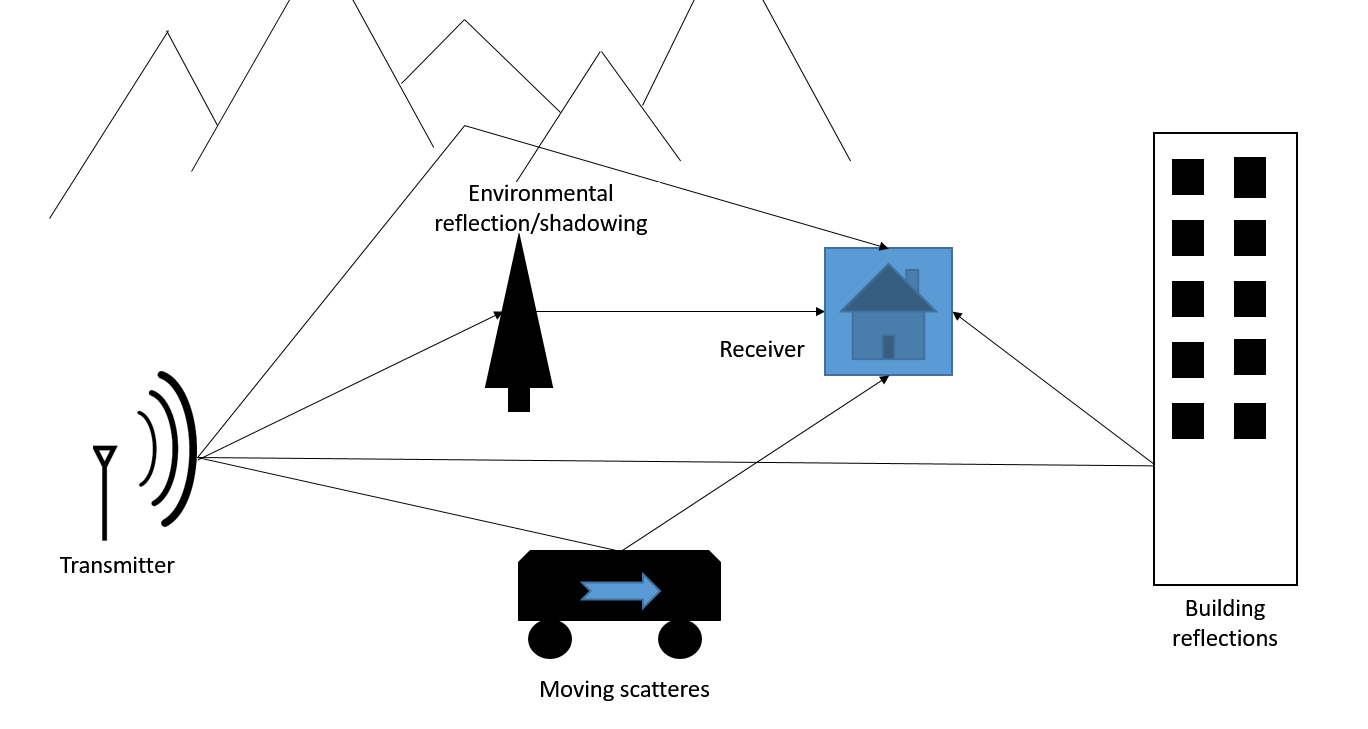
\includegraphics[width=0.95\textwidth]{reflections.png}
	\caption{Interferences in a normal transmission between two devices}
	\label{fig:interferences}
\end{figure}
\newpage
\subsection{AWGN Channel}
\label{AWGN}

The easiest kind of channel manipulation is to add random Gaussian noise to the channel, also commonly known as an \gls{AWGN} channel. Like the name says we will add noise, which is a random Gaussian distribution with flat spectral density, to an existing transmitted signal.
First of all a definition for \acrfull{SNR} is given:
\begin{equation}
\label{eq:SNR}
\textrm{SNR} = \frac{\E[{\lvert X \rvert}^2]}{\E[{\lvert N \rvert}^2]} = \frac{\sigma_{x}^2}{1},
\end{equation}
Second the probability density function of a Gaussian distribution need to be defined:
\begin{equation}
\label{eq:AWGNpdf}
P_{Y|X}(y|x) = \frac{1}{\pi\sigma^2}e^{-\frac{(y-x)^2}{\sigma^2}},  
\end{equation}
Our receiver will receive a signal like this:
\begin{equation}
\label{eq:1.1}
Y = X + N ,
\end{equation}
with Y being the received symbols, X $\sim \mathcal{N}_c(0,\sigma_{x}^2)$ the send symbol and N $\sim \mathcal{N}_c(0,1)$ the complex AWGN noise. This can be applied for a full transmission of messages resulting in:
\begin{equation}
\label{eq:1.2}
\underline{Y} = \underline{X} + \underline{N},
\end{equation}
which can be depicted more detailed like this:
\begin{equation}
\label{eq:1.3}
[Y_1,Y_2,...,Y_n] = [X_1,X_2,...,X_n] + [N_1,N_2,...,N_n],
\end{equation}
the lowercase n noting the length of the code word.
with y being the acquired point,x the transmitted symbol and $\sigma^2$ the variance of the distribution.
Gaussian noise, representing thermal noise and overlay with multiple users in a wireless system, is therefore used in all the simulations run in this thesis. In \fig{fig:AWGNSP} a depiction of the spectral power distribution of \gls{AWGN}.
\begin{figure}[!htb]
	\centering
	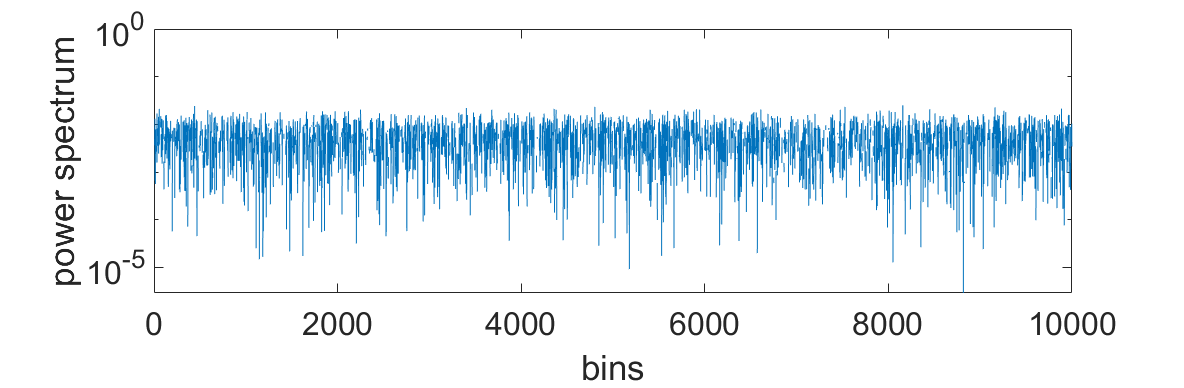
\includegraphics[width=0.95\textwidth]{AWGN.png}
	\caption{Power spectral density in a AWGN channel}
	\label{fig:AWGNSP}
\end{figure}
\newpage
\subsection{Rayleigh Fading Channel}
\label{sec:rayleigh}
Another common channel model used in communication theory is Rayleigh fading. Rayleigh fading simulates multi path reception, which means that for a receiver antenna in a wireless link there are many reflected and scattered signals reaching it (\fig{fig:interferences}). These kind of reflections are often seen in high-density urban areas. This results in construction or destruction of signal waves. The channel will now look like this:
\begin{equation}
\label{eq:rayleigh1}
Y = HX + N,  
\end{equation}
which adds the new fading coefficient H to the transmitted message.
\newline
As shown before in the \gls{AWGN} channel the above \eq{eq:rayleigh1} can be expanded for a full transmission. Before that it needs to be clarified that not every symbol will be multiplied with a different fading coefficient H, but a whole block of symbols. This kind of transmission with Rayleigh fading is known as block fading:
\begin{equation}
\label{eq:rayleigh2}
[Y_1,...,Y_{kT}] = [H_1X_1,...,H_1X_T]...[H_kX_{(K-1)T+1},...,H_kX_{kT}] + [N_1,...,N_{kT}] \textrm{ , } kt = n,  
\end{equation}
with the subscript $T$ indicating the length of the block, $k$ the number of blocks in a codeword and $n$ the length of the codeword. The block length can be chosen ranging from on single symbol up to the whole code word being one block.
\newline
The graphic (\fig{fig:rayleigh}) shows the power distribution over 12000 samples. Being Gaussian randomly distributed there are now these so called "deep fadings" where the power of the fading drops, which will also decrease the signal power of the received signal to drop significantly. This results in the so-called burst errors, which were mentioned in Chapter \eref{sec:interleaver}.
\begin{figure}[!htb]
	\centering
	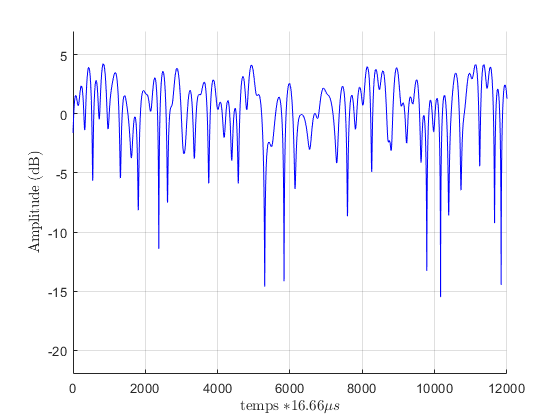
\includegraphics[width=0.95\textwidth]{rayleigh.png}
	\caption{Power spectral density in a Rayleigh channel}
	\label{fig:rayleigh}
\end{figure}